\documentclass[dvipdfmx,12pt]{beamer}

\usepackage{bxdpx-beamer}
\usepackage{pxjahyper}
\usepackage{minijs}
\usetheme{Annarbor}
\usepackage{mathpazo}
\usepackage{amsmath,amssymb}
\usepackage{graphicx}
\usepackage{array}

\title{Dunne, Roberts \& Samuelson \\(1988, RAND)}
\subtitle{Patterns of firm entry and exit \\ in U.S. manufacturing industries}
\author{Reio TANJI}
\date{July.4th,2018}
\institute{Osaka University}

\begin{document}
\begin{frame}\frametitle{}
\titlepage
\end{frame}


\section*{A Table of Contents}
\begin{frame}\frametitle{Contents}
\tableofcontents
\end{frame}

\section{Introduction}
\begin{frame}\frametitle{Abstract}

 \begin{itemize}
 
 \item Summerizes the pattern of firm, entry and exit in the four-digit U.S. manufacturing industries over the period 1963-1982.
 
 \item Sorting entrants by the type of entry, and examine the relative importance of each types
 
 : entry-exit rates, and postentry performance
 
 \end{itemize}

\end{frame}

\begin{frame}\frametitle{Background}

 \begin{itemize}
 
 \item Theoretical studies have examined the of deterring entry.
 
 \item Empirical studies have investigated the correlation between variables measuring market performance and factors that can hinder the entry.
 
 \item This paper provide the stylized facts about the actual patterns of firm entry and exit in the U.S. economy.
 
 \end{itemize}

\end{frame}

\begin{frame}\frametitle{Attention}

 \begin{itemize}
 
 \item They focused on three aspects of the entry and exit process.
 
  \begin{enumerate}
  
  \item Types of entrants
  
  : whether the entrant is a newly established firm or not, and whether the firm constructed a new plant to produce goods for entry to the industry.
  
  \item Time-series and cross-industres patterns of entry-exit behavior
  
  \item Postentry performance of the entrants
  
  : market shares, average size, and failure rate as they age  
  
  \end{enumerate}
 
 \end{itemize}

\end{frame}

\section{Data}
\begin{frame}\frametitle{Data}

 \begin{itemize}
 
 \item Dataset : Constructed from U.S. Census Bureau 
 
 covers all firms producing each four-digit manufacturing industries in 1963, 1967, 1972, 1977, and 1982.
 
 \item Two general approaches in studies on firm/industry evolution : industry level and firm level.
 
 - This paper uses \textbf{individual plant-level} data.
 
 \end{itemize}

\end{frame}

\begin{frame}\frametitle{Data Construction}

 \begin{itemize}
 
 \item Standardization
 
 Reclassfied seven-digit census in `63 and `67 into the proper four-digit industry.
 
 \item Matching
 
 Sale of the plant or legal reorganizations(administrative changes) may change plants' ID number, which leads to overstate entry and exit.
 
 $\Rightarrow$ To get rid of these measurement errors, they exclude the extremely small firms.
 
 \end{itemize}
 
\end{frame}

\begin{frame}\frametitle{Data Construction}

 \begin{itemize}
 
 \item Aggregation
 
 Construct firm-level data from the plant-level data
 
 : Distinguish firms with single-plant with multiplant
 
 $\Rightarrow$ Single-plant firms account for 93.4\% of the total number, but 17.2 \% of the value of production.
 
 \item Identification
 
  \begin{itemize}
  
  \item Year of Entry
  
  \item Entry Type
  
  New firm and diversifyng firm
  
  \item Entry Method
  
  New plant construction and changing the mix of products
  
  \end{itemize}
 
 \end{itemize}

\end{frame}

\begin{frame}

\begin{center}

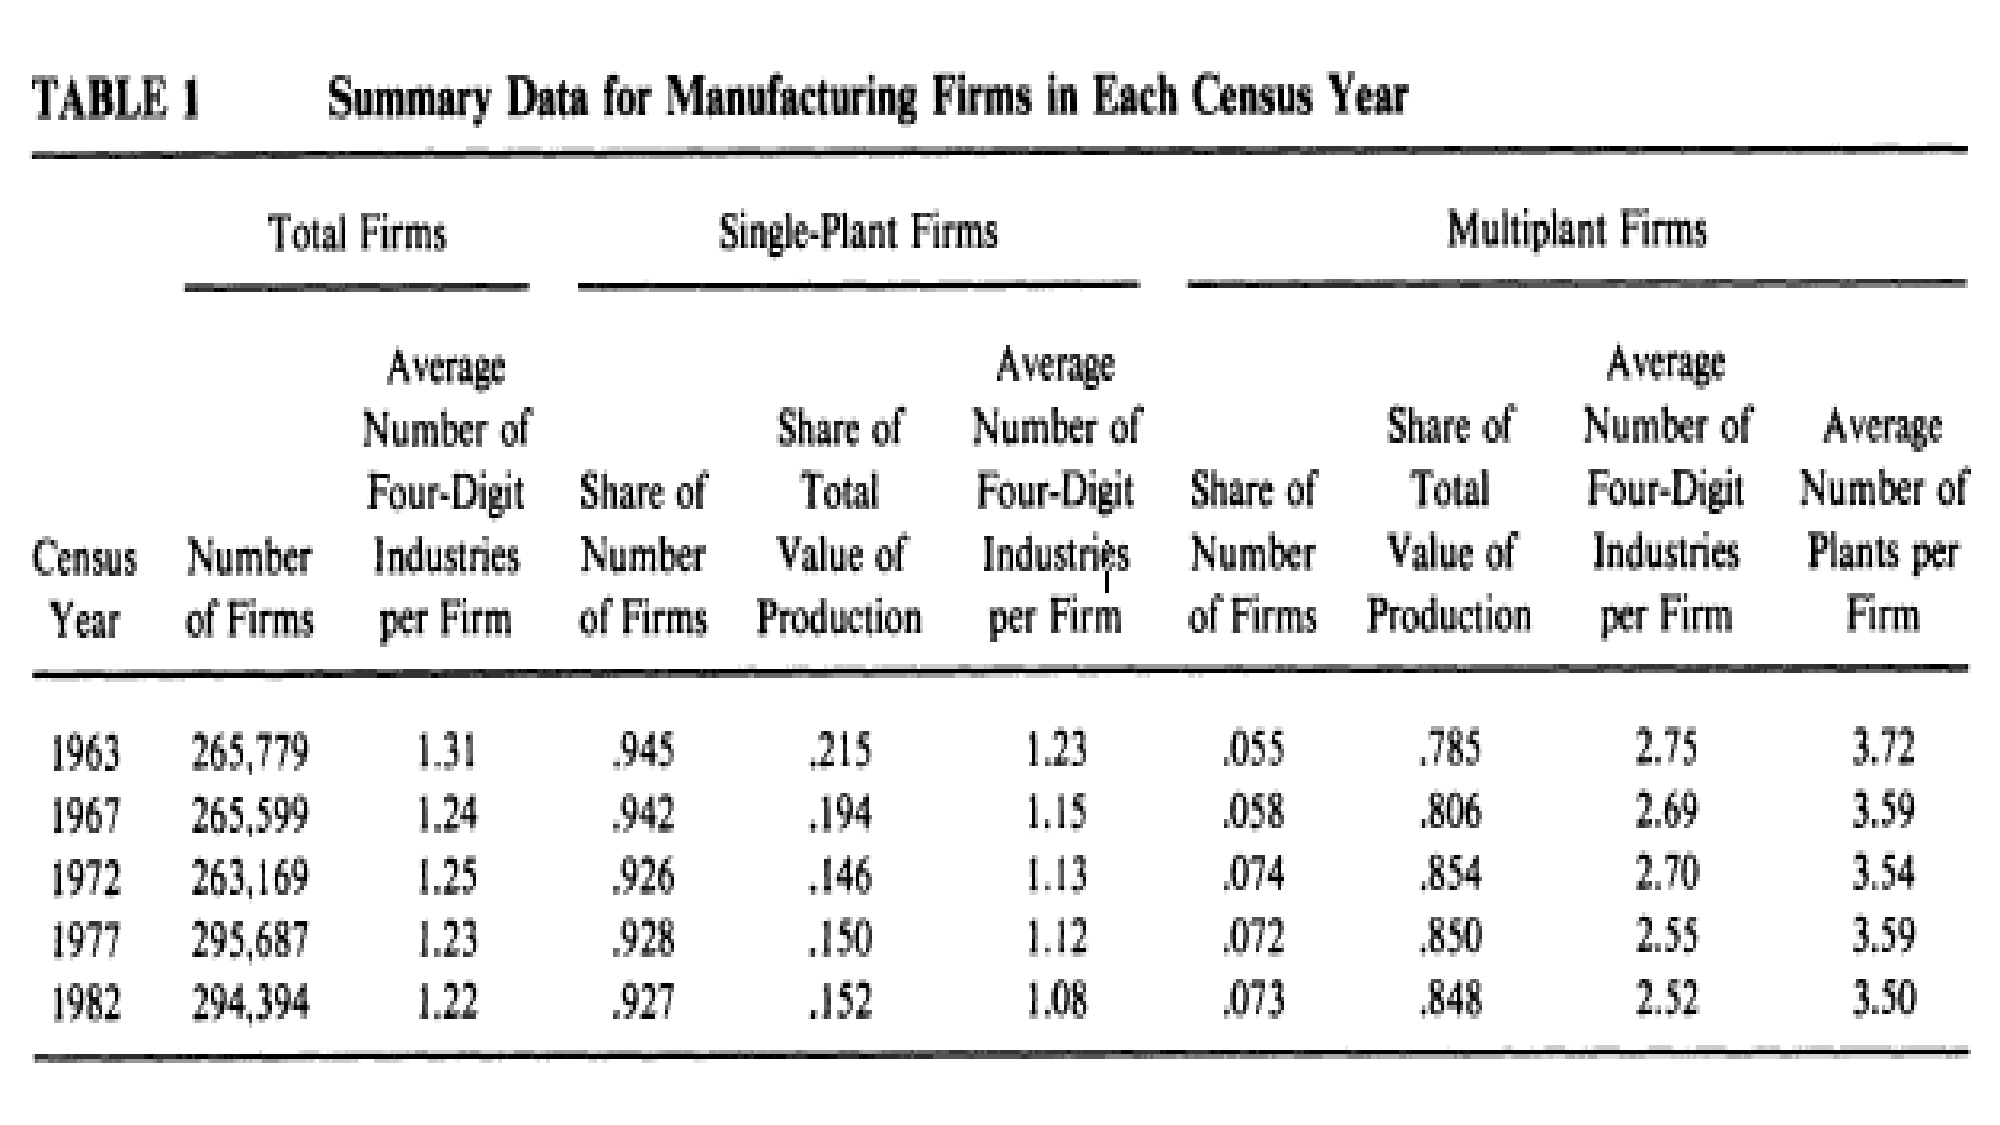
\includegraphics[width=12cm,height=5.5cm]{DRS_T1.pdf}

\end{center}

\end{frame}

\begin{frame}\frametitle{Entry \& Exit Measures}

\footnotesize

 \begin{itemize}
 
 \item Entry and Exit Rates :
 
  \begin{align*}
  ER_i(t) &= NE_i(t)/NT_i(t-1) \\
  XR_i(t-1) & = NX_i(t-1) / NT_i(t-1)
  \end{align*} 
 
 \item Market Shares :
 
  \begin{align*}
  ESH_i(t) &=QE_i(t)/QT_i(t-1) \\
  XSH_i(t-1) &= QX_i(t-1) / QT_i(t-1)
  \end{align*}
 
 \item Average Size : average output per firm
 
  \begin{align*}
  ERS_i(t) &= \dfrac{QE_i(t)/NE_i(t)}{(QT_i-QE_i(t))/(NT_i(t) - NE_i(t))} \\
  XRS_i(t-1) &=\dfrac{QX_i(t)/NX_i(t-1)}{(QT_i(t-1)-QX_i(t-1))/(NT_i(t-1)-NX_i(t-1))}
  \end{align*}
 
 \end{itemize}

\large

\end{frame}

\section{Average entry and exit statistics}
\begin{frame}\frametitle{Importance of Entrants/Entry Types}

 \begin{itemize}
 
 \item In each census years, 30-40 \% of the firms are entrants.
 
 \item Their market shares and sizes are relatively small (15.8\% and 35.2\% on average, respectively). 
 
 \item Exit variables reveal a similar pattern.
 
 \item New-firm, new-plant (NF/NP) account for more than half rate of number among the entrants, followed by diversifying-firm, existing-plants(DF/PM)(36.1\%) and diversifying-firm, new-plant(DF/NP)(8.5\%).
  
 \end{itemize}

\end{frame}

\begin{frame}

\begin{center}

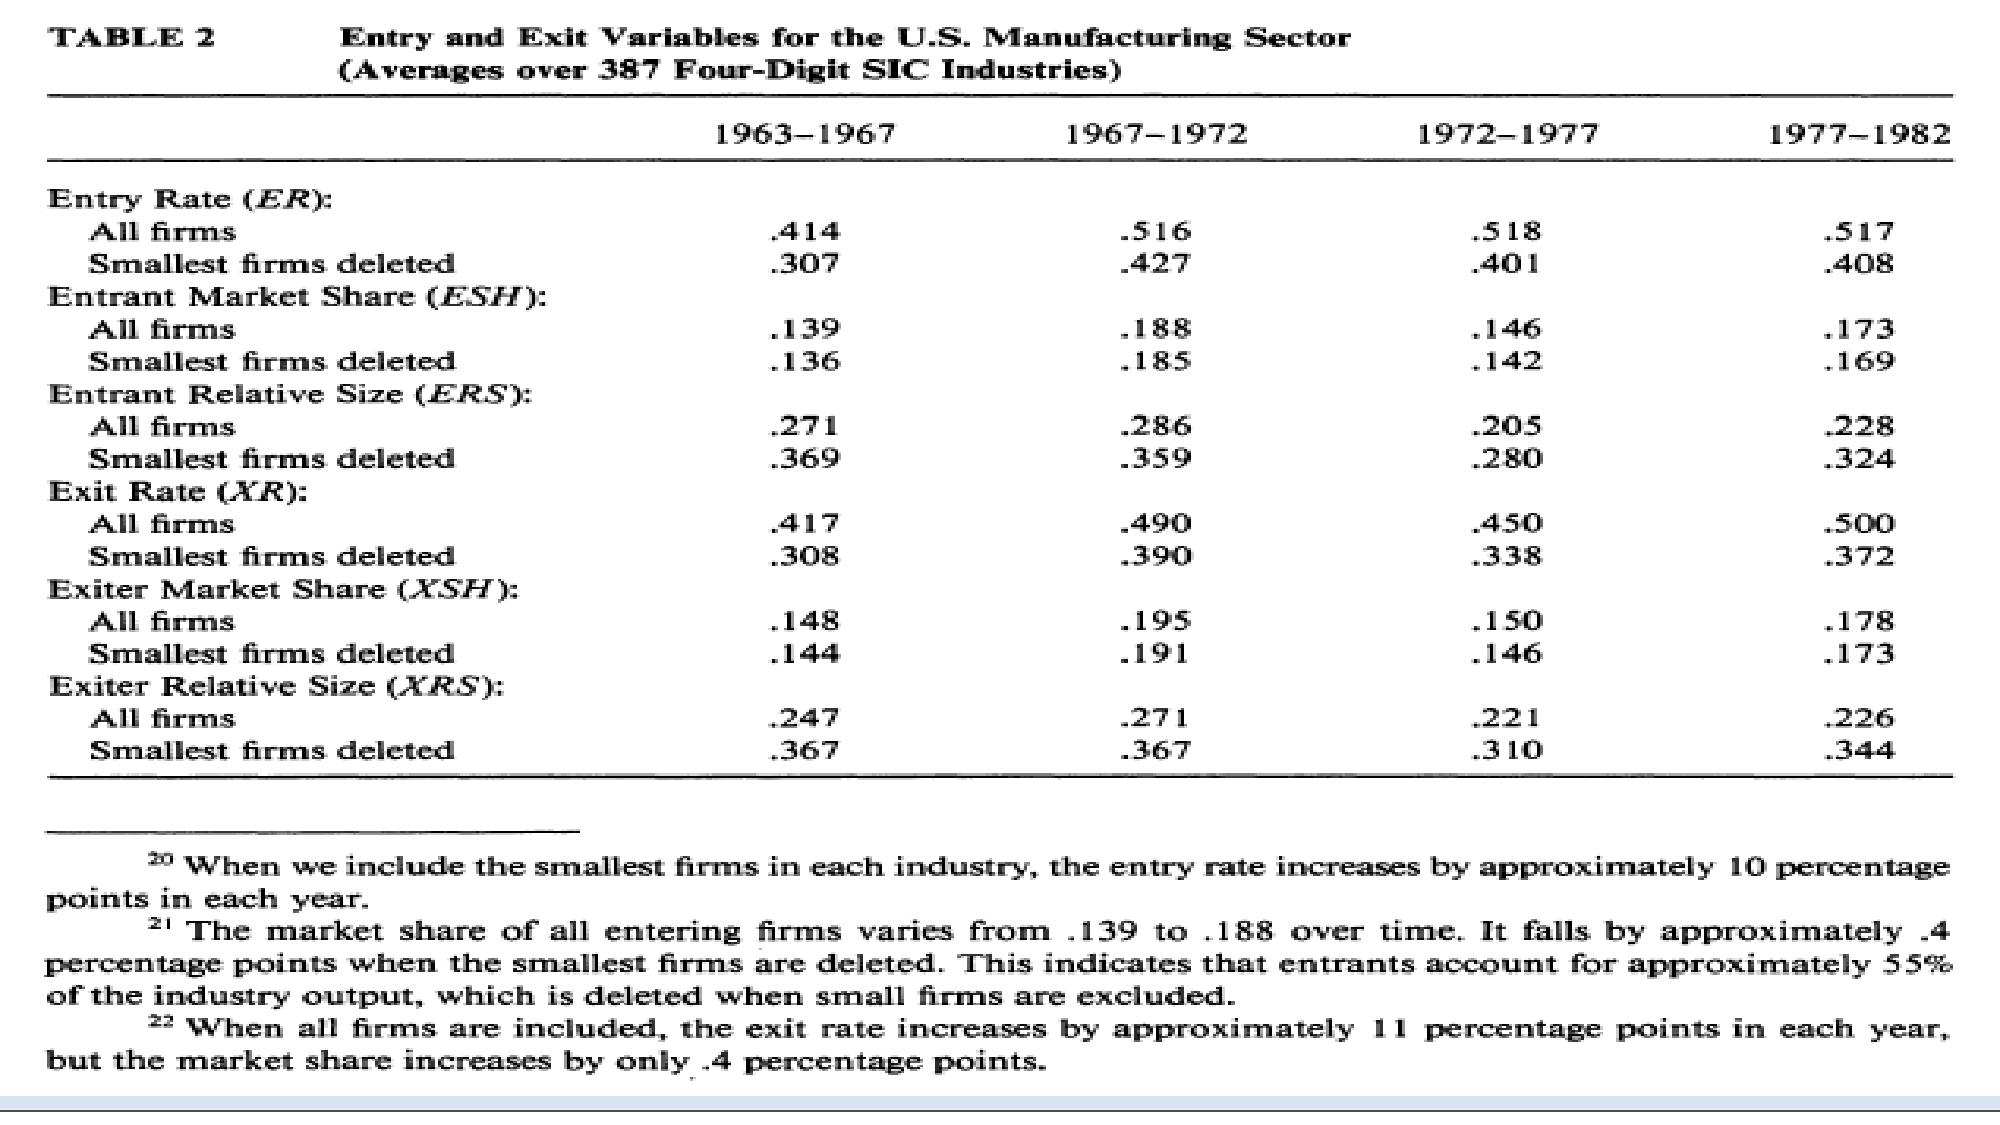
\includegraphics[width=9cm,height=7.75cm]{DRS_T2.pdf}

\end{center}

\end{frame}

\begin{frame}

\begin{center}

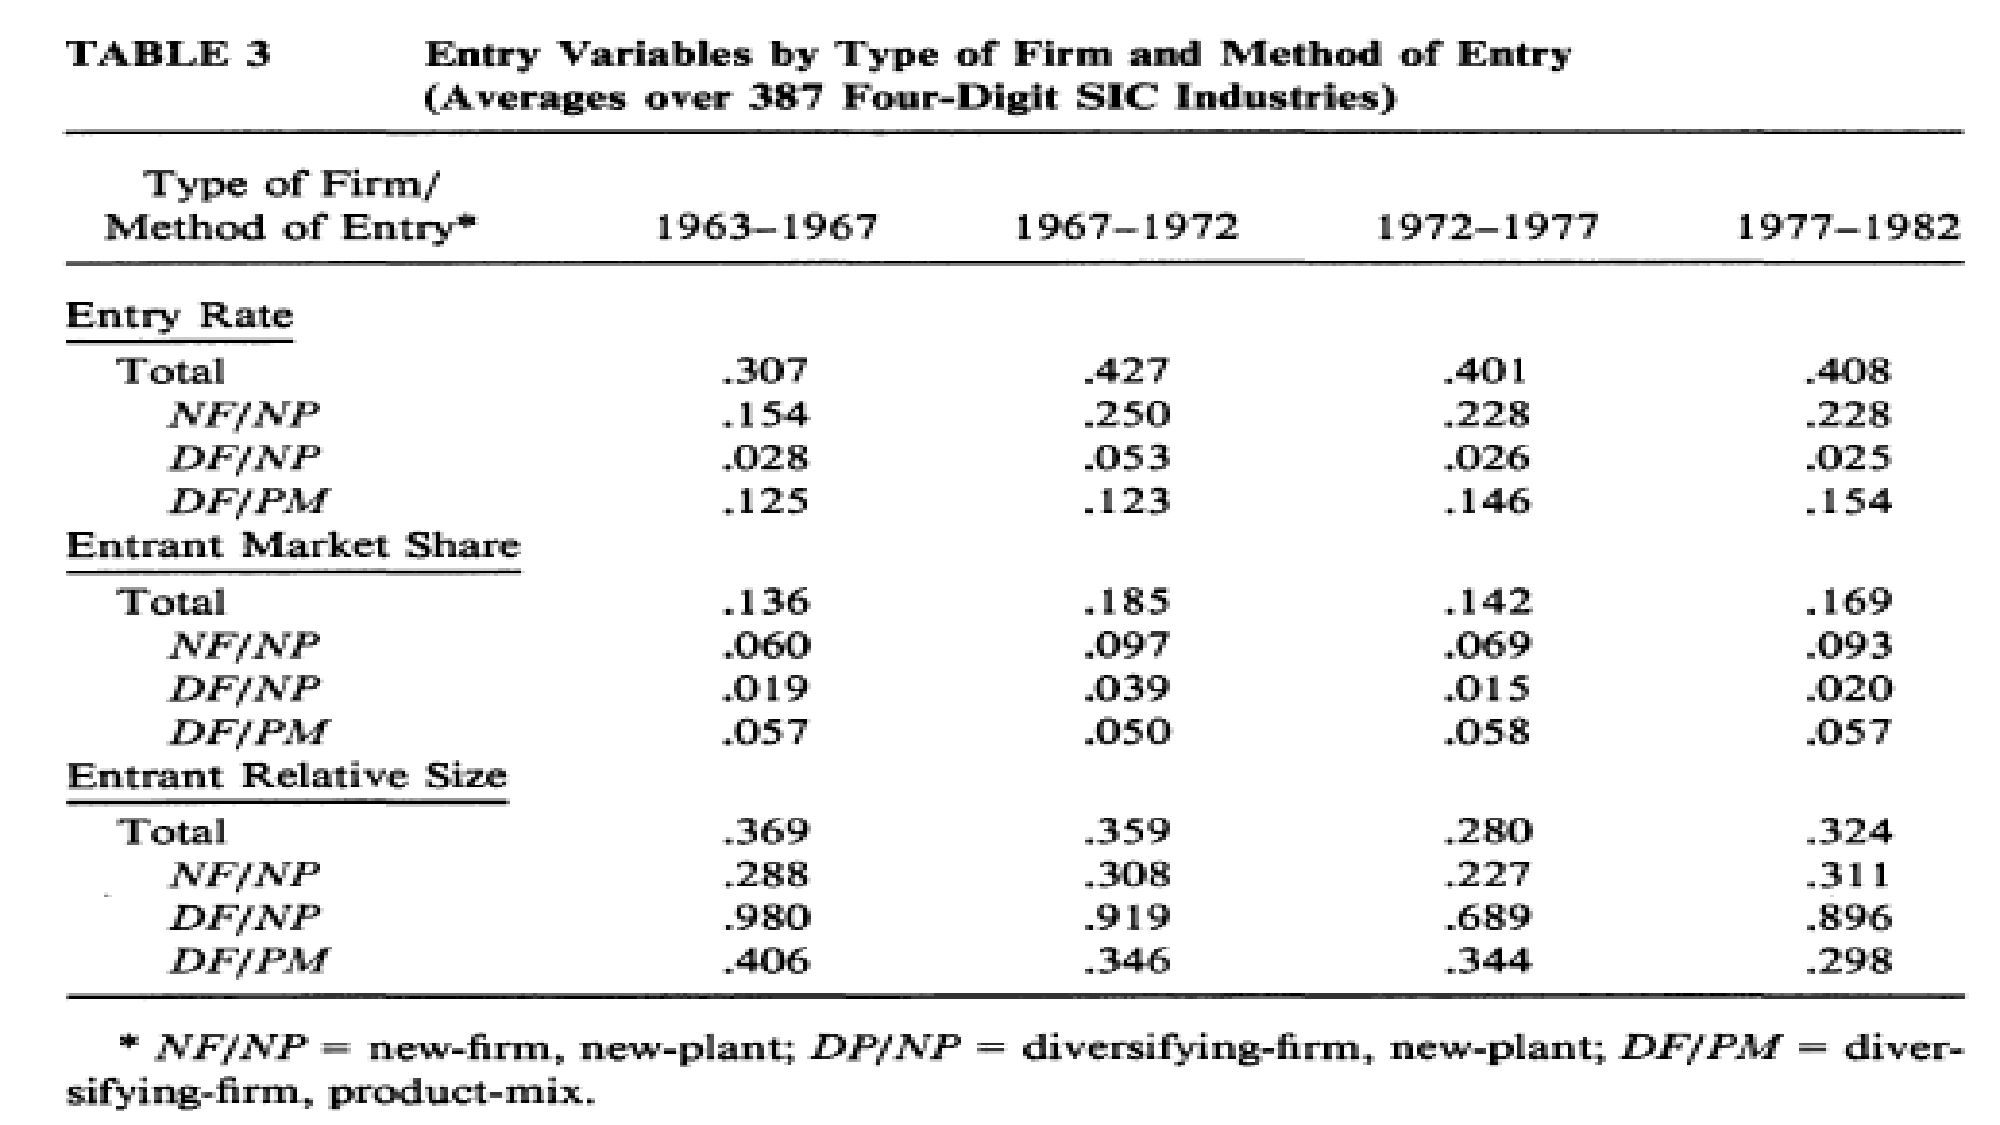
\includegraphics[width=9cm,height=7.75cm]{DRS_T3.pdf}

\end{center}

\end{frame}

\begin{frame}

\begin{center}

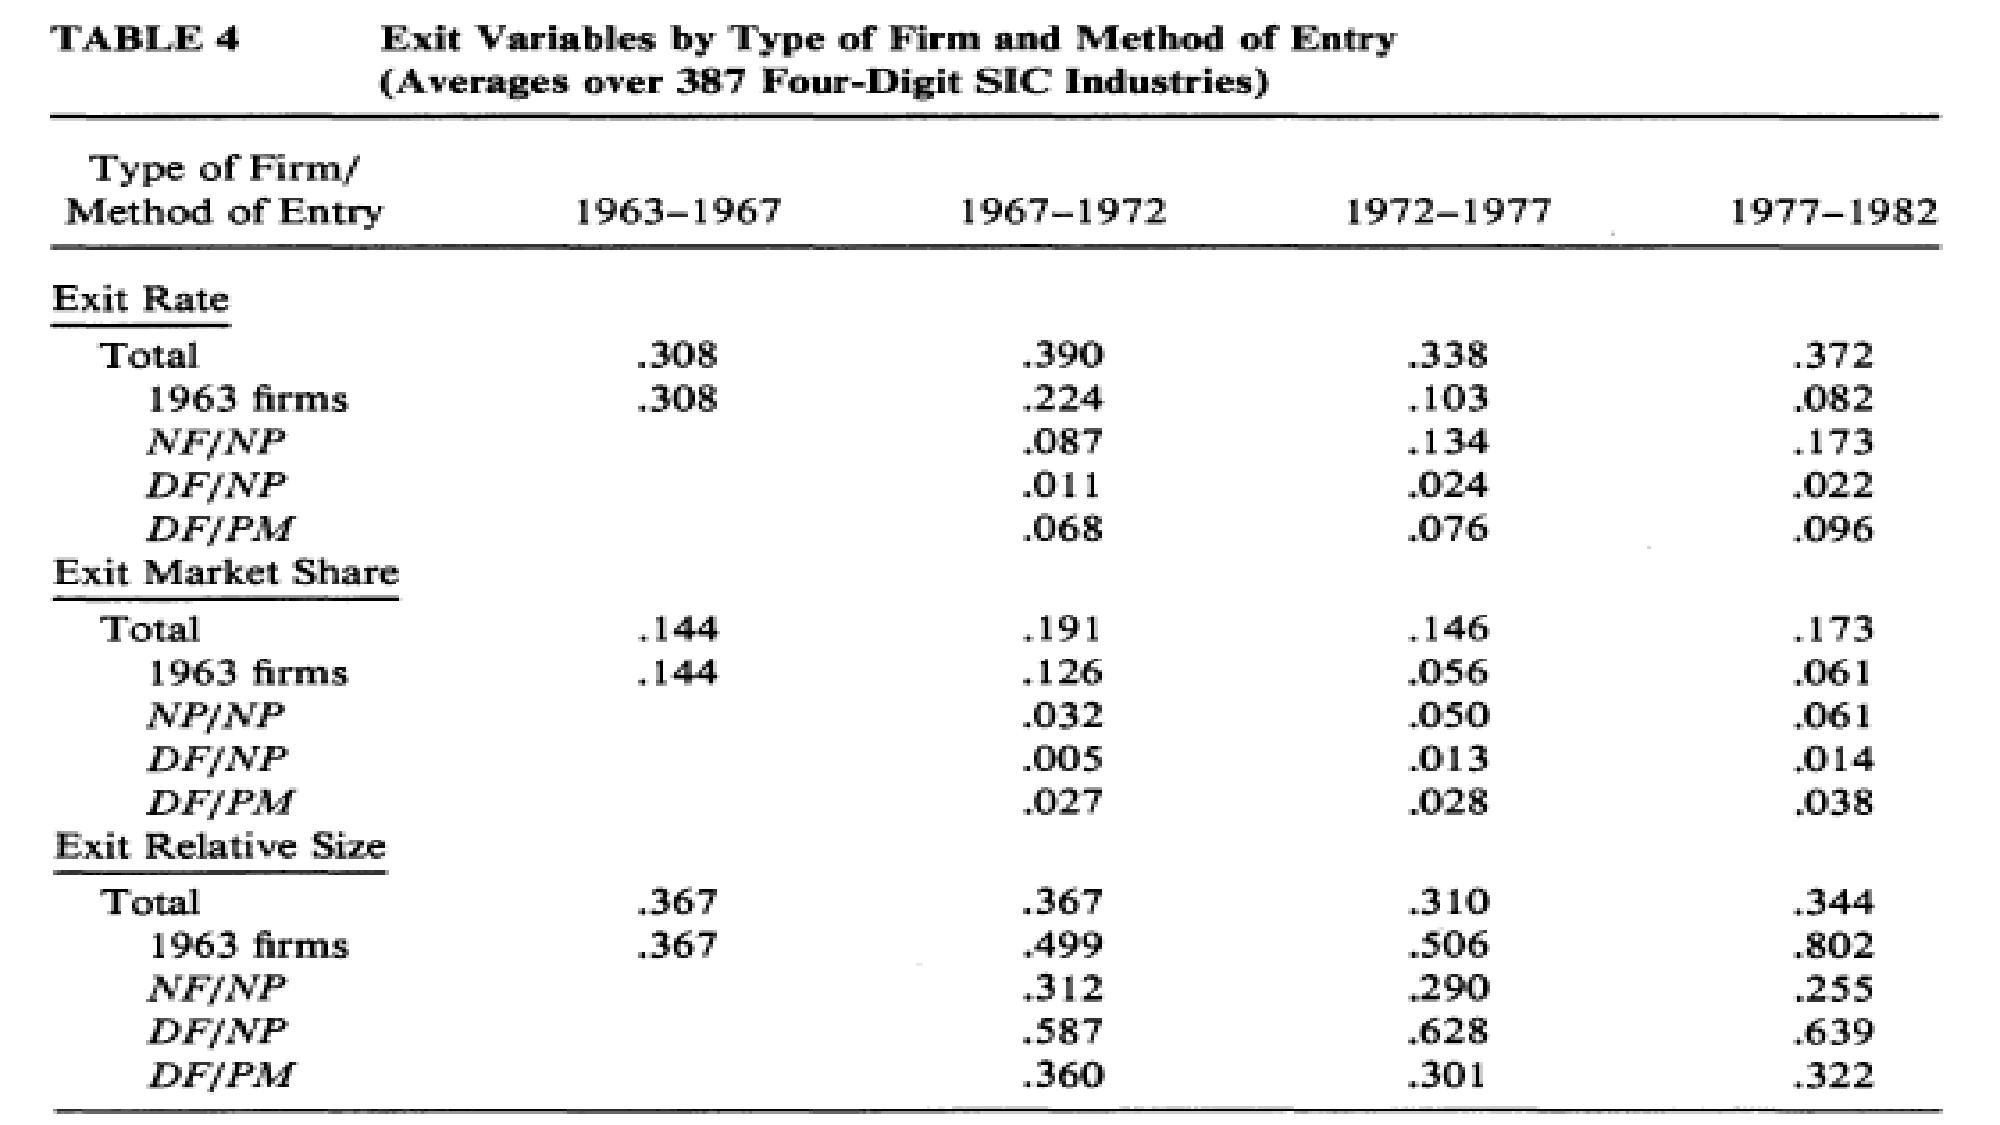
\includegraphics[width=9cm,height=7.75cm]{DRS_T4.pdf}

\end{center}

\end{frame}

\section{Variation in Industry Entry and Exit Patterns}
\begin{frame}\frametitle{Across Industries}

 \begin{itemize}
 
 \item Across-industry difference is substantial.
 
  \begin{itemize}
  
  \item In each sector, there exists an industry whose entry rate is extremely high/low.
  
  \end{itemize}
 
 \item Generally, the entrants' effect on their industry's output is small.
 
 \item Sector-charactaristics of the exit firms are similar to that of the entrants.
 
 - The simple correlation of average market share is .92.
 
 - That of average relative size is .98.
 
 \end{itemize}

\end{frame}

\begin{frame}

\begin{center}

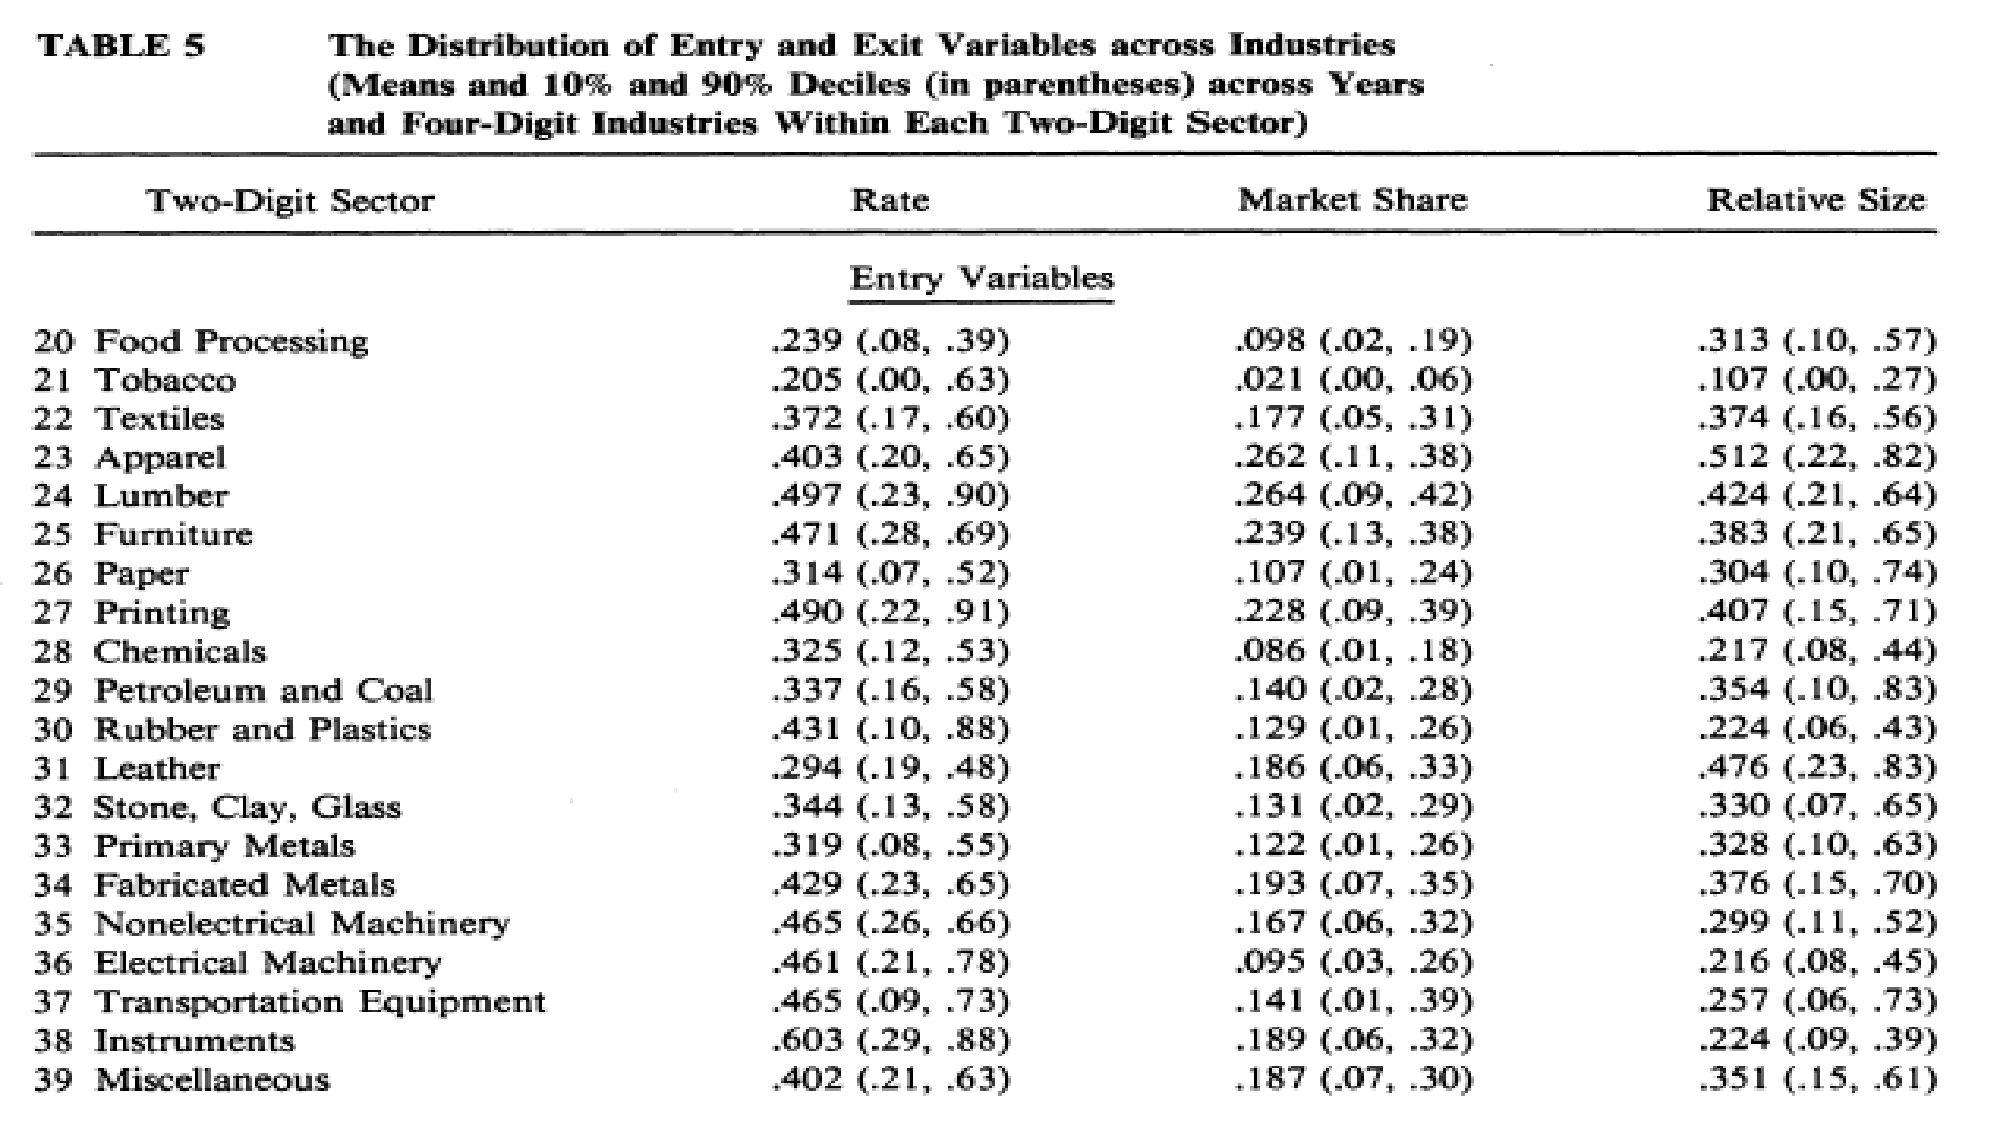
\includegraphics[width=9.5cm,height=7.75cm]{DRS_T5a.pdf}

\end{center}

\end{frame}

\begin{frame}

\begin{center}

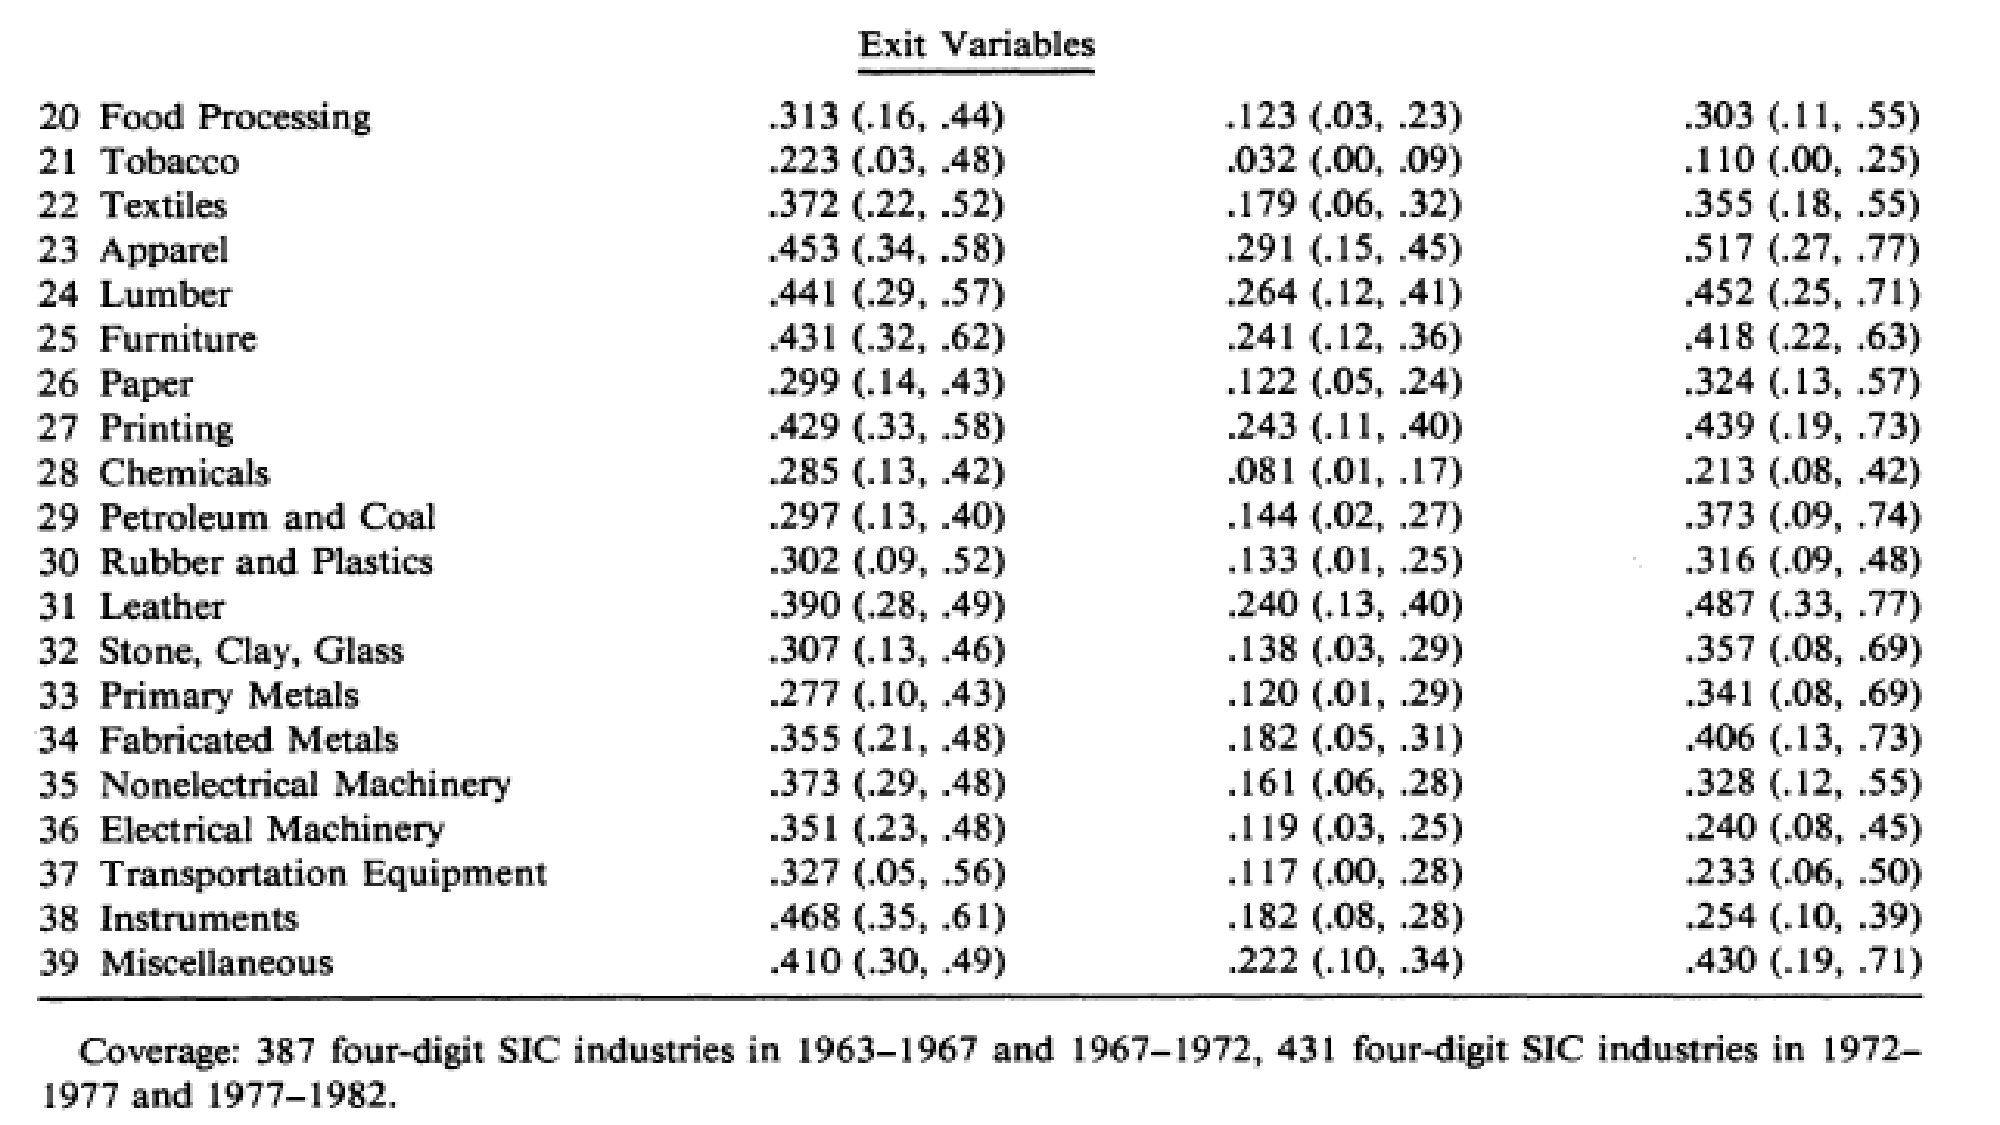
\includegraphics[width=10.5cm,height=7.75cm]{DRS_T5b.pdf}

\end{center}

\end{frame}

\begin{frame}\frametitle{Time-Series Correlation}

 \begin{itemize}
 
 \item Each variables are positively correlates with itself across census years, especially in market share.
 
  : Correlation diminishes as the years become farther apart.
 
 \item Industries with high entry rate also tend to have high rate of exits.
 
 \item Considering panel nature :  considering industry-specific characters, the correlation between entry-exit rate(deviation from the industry mean) in the same period is negative.

- $t$ period and $t+1$ period are positively correlated.
 
 \item About market share, such charactaristics are not observed.
 
 \end{itemize}

\end{frame}

\begin{frame}

\begin{center}

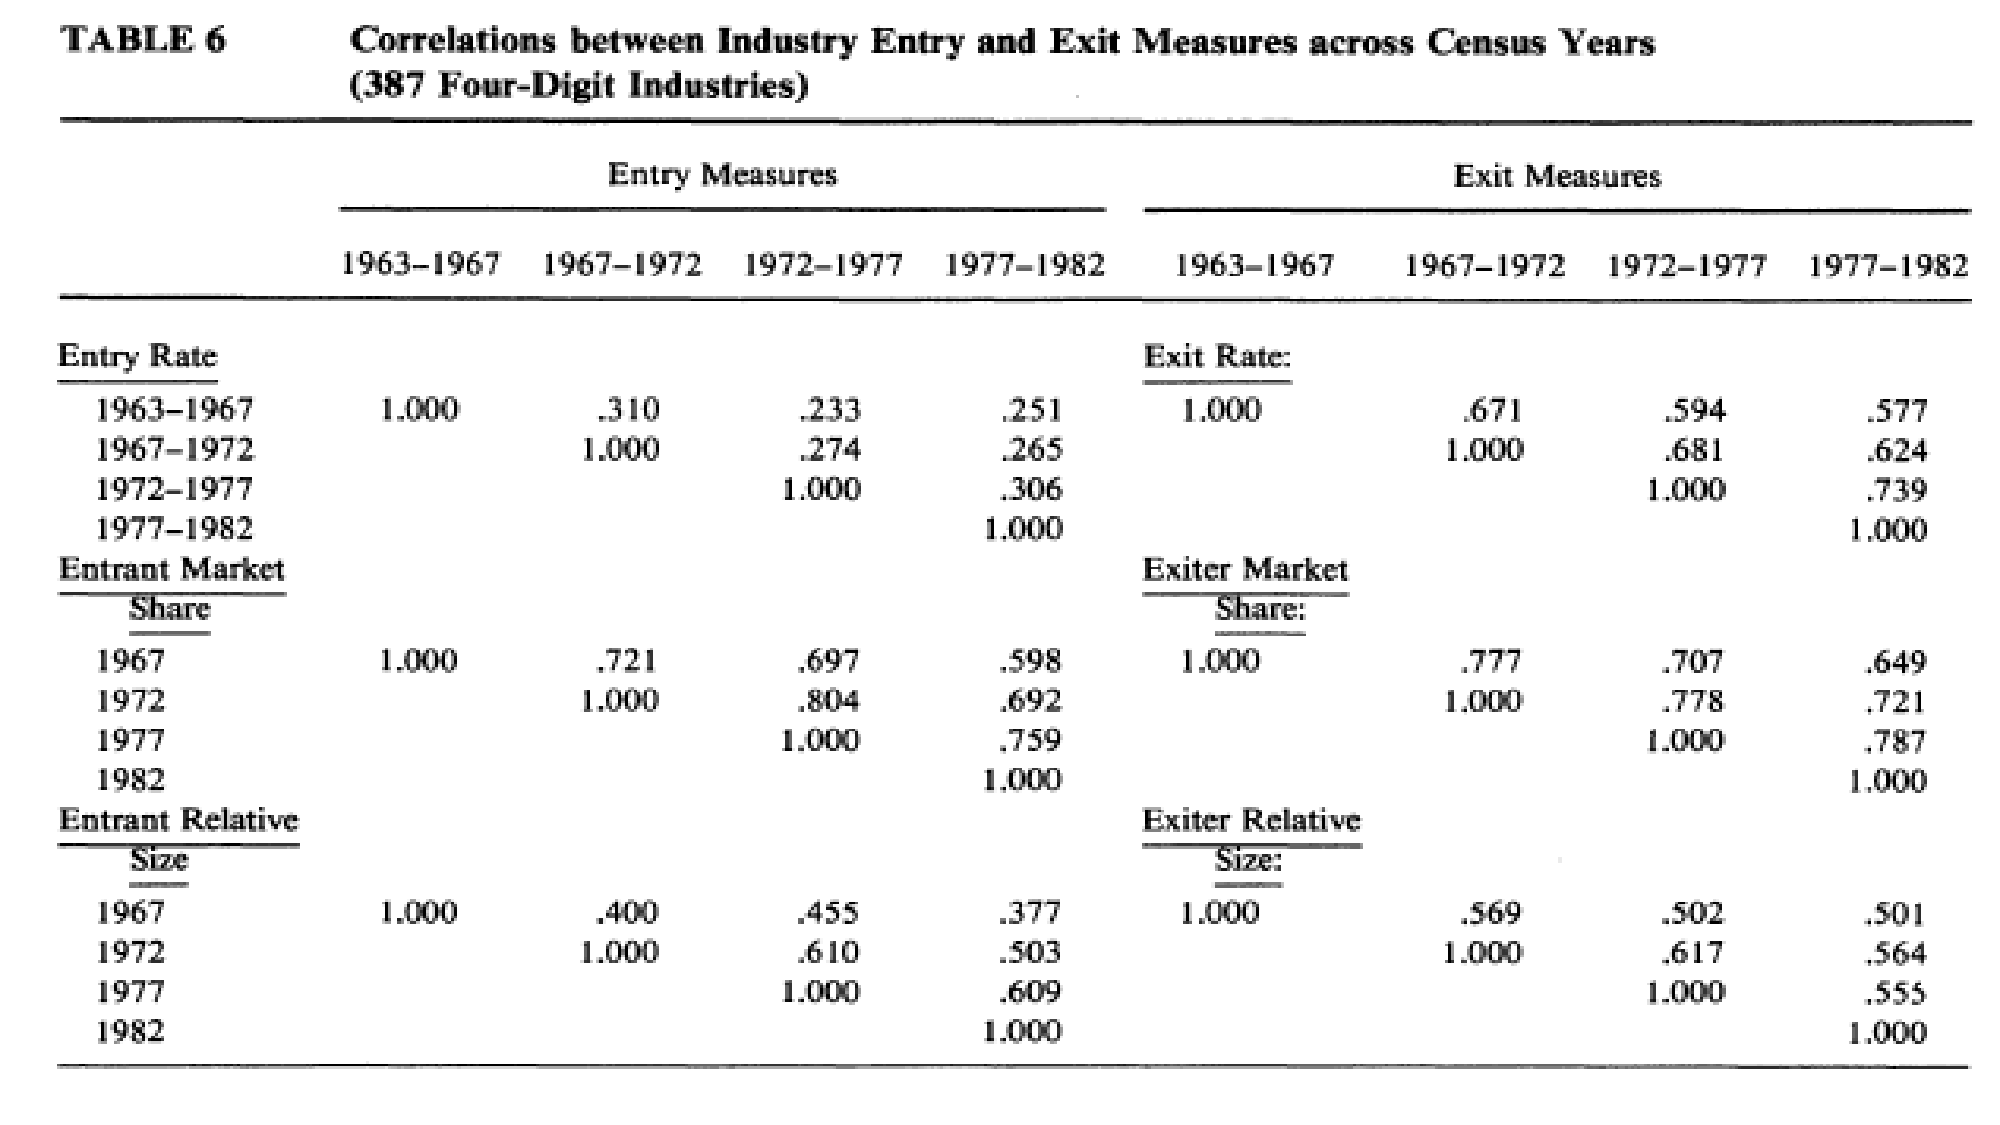
\includegraphics[width=10cm,height=7.75cm]{DRS_T6.pdf}

\end{center}

\end{frame}

\begin{frame}

\begin{center}

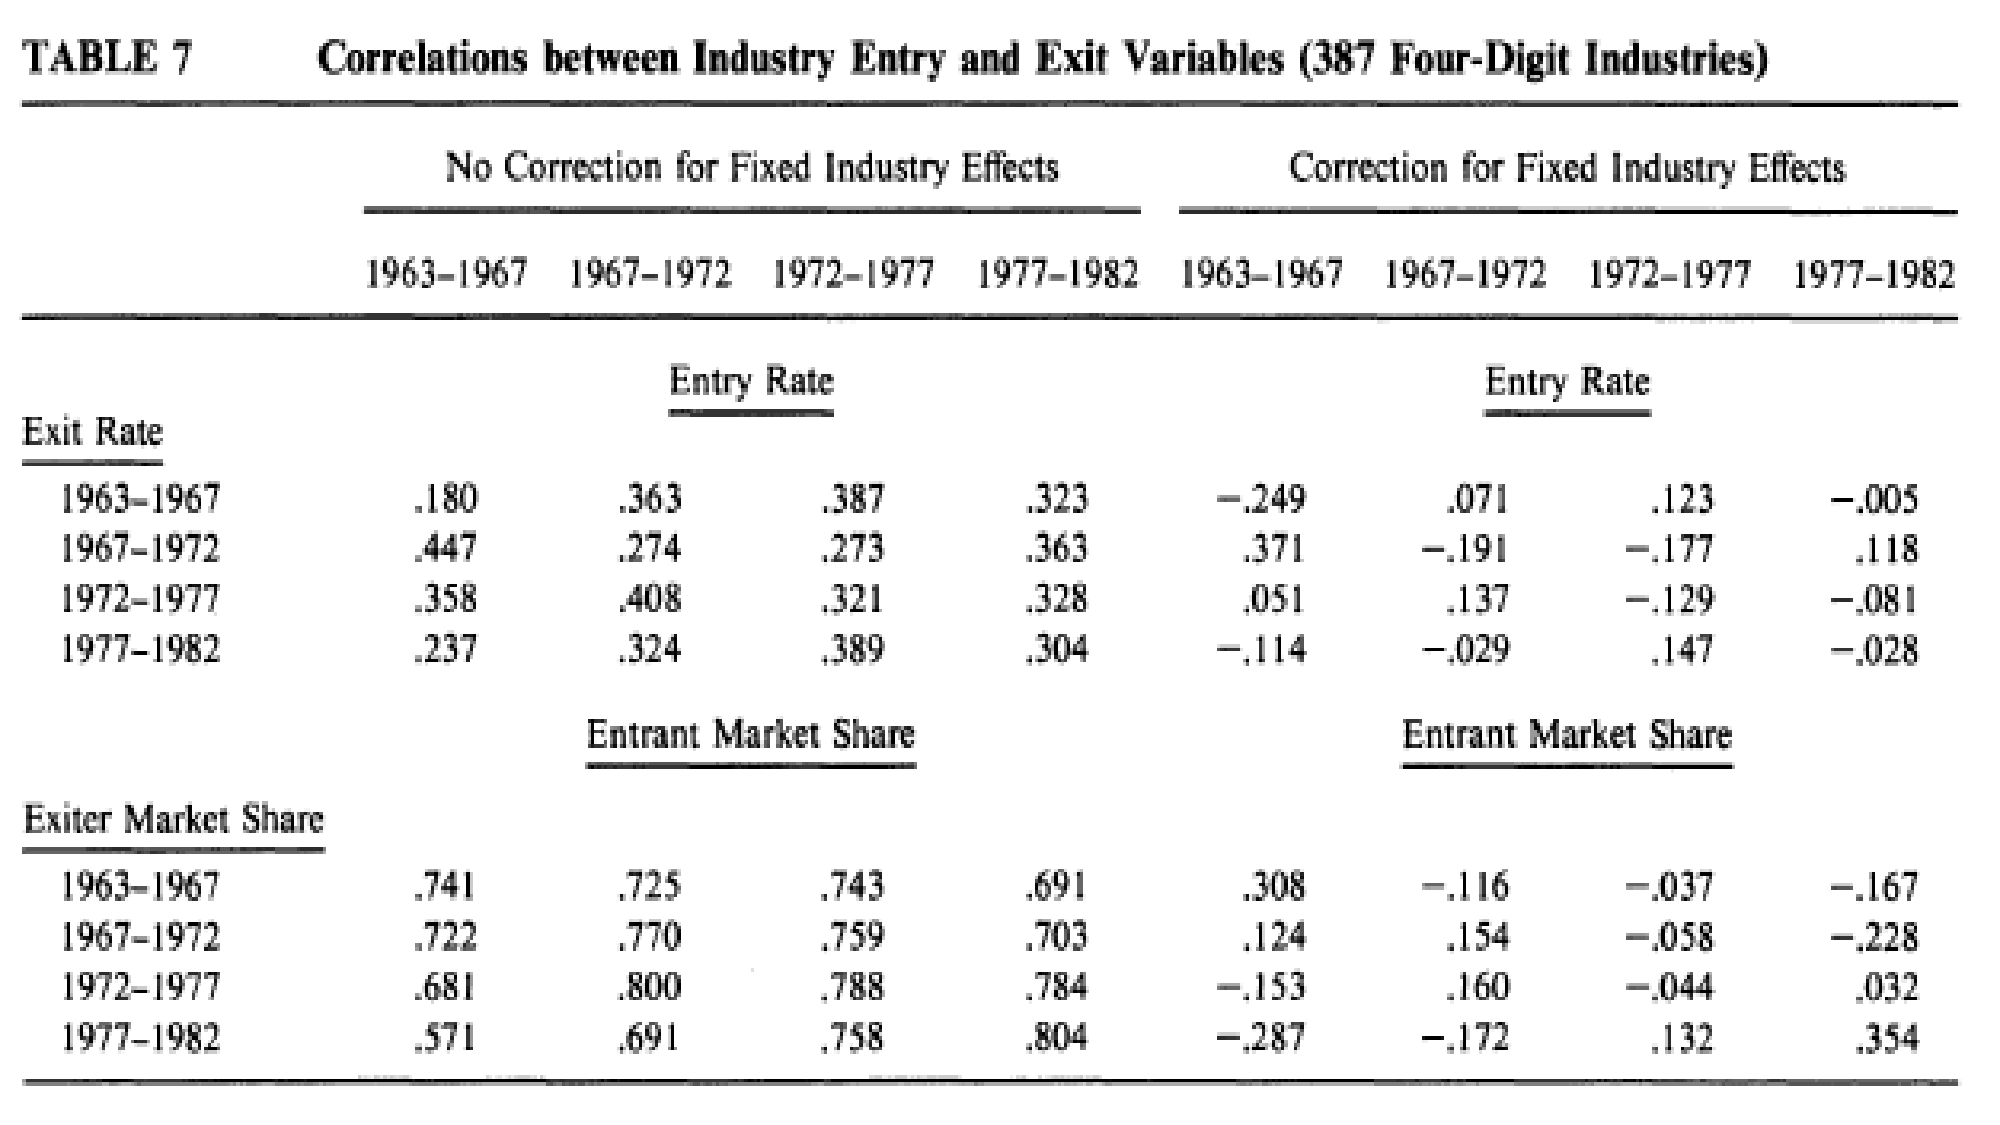
\includegraphics[width=11.5cm,height=7.5cm]{DRS_T7.pdf}

\end{center}

\end{frame}

\section{Longitudial Aspects of Entry and Exit}
\begin{frame}\frametitle{Growth and Exit of the Entrants}

 \begin{itemize}
 
  \item After the entry, the entrants' market share tend to decline as time goes.
  
  : Exit of firms
  
  \item Average size continues to increase
  
  : Surviving firms grow as the cohort ages.
 
 \item On average, 79.6 \% of all firms exit within 10 years.
 
 \end{itemize}

\end{frame}

\begin{frame}

\begin{center}

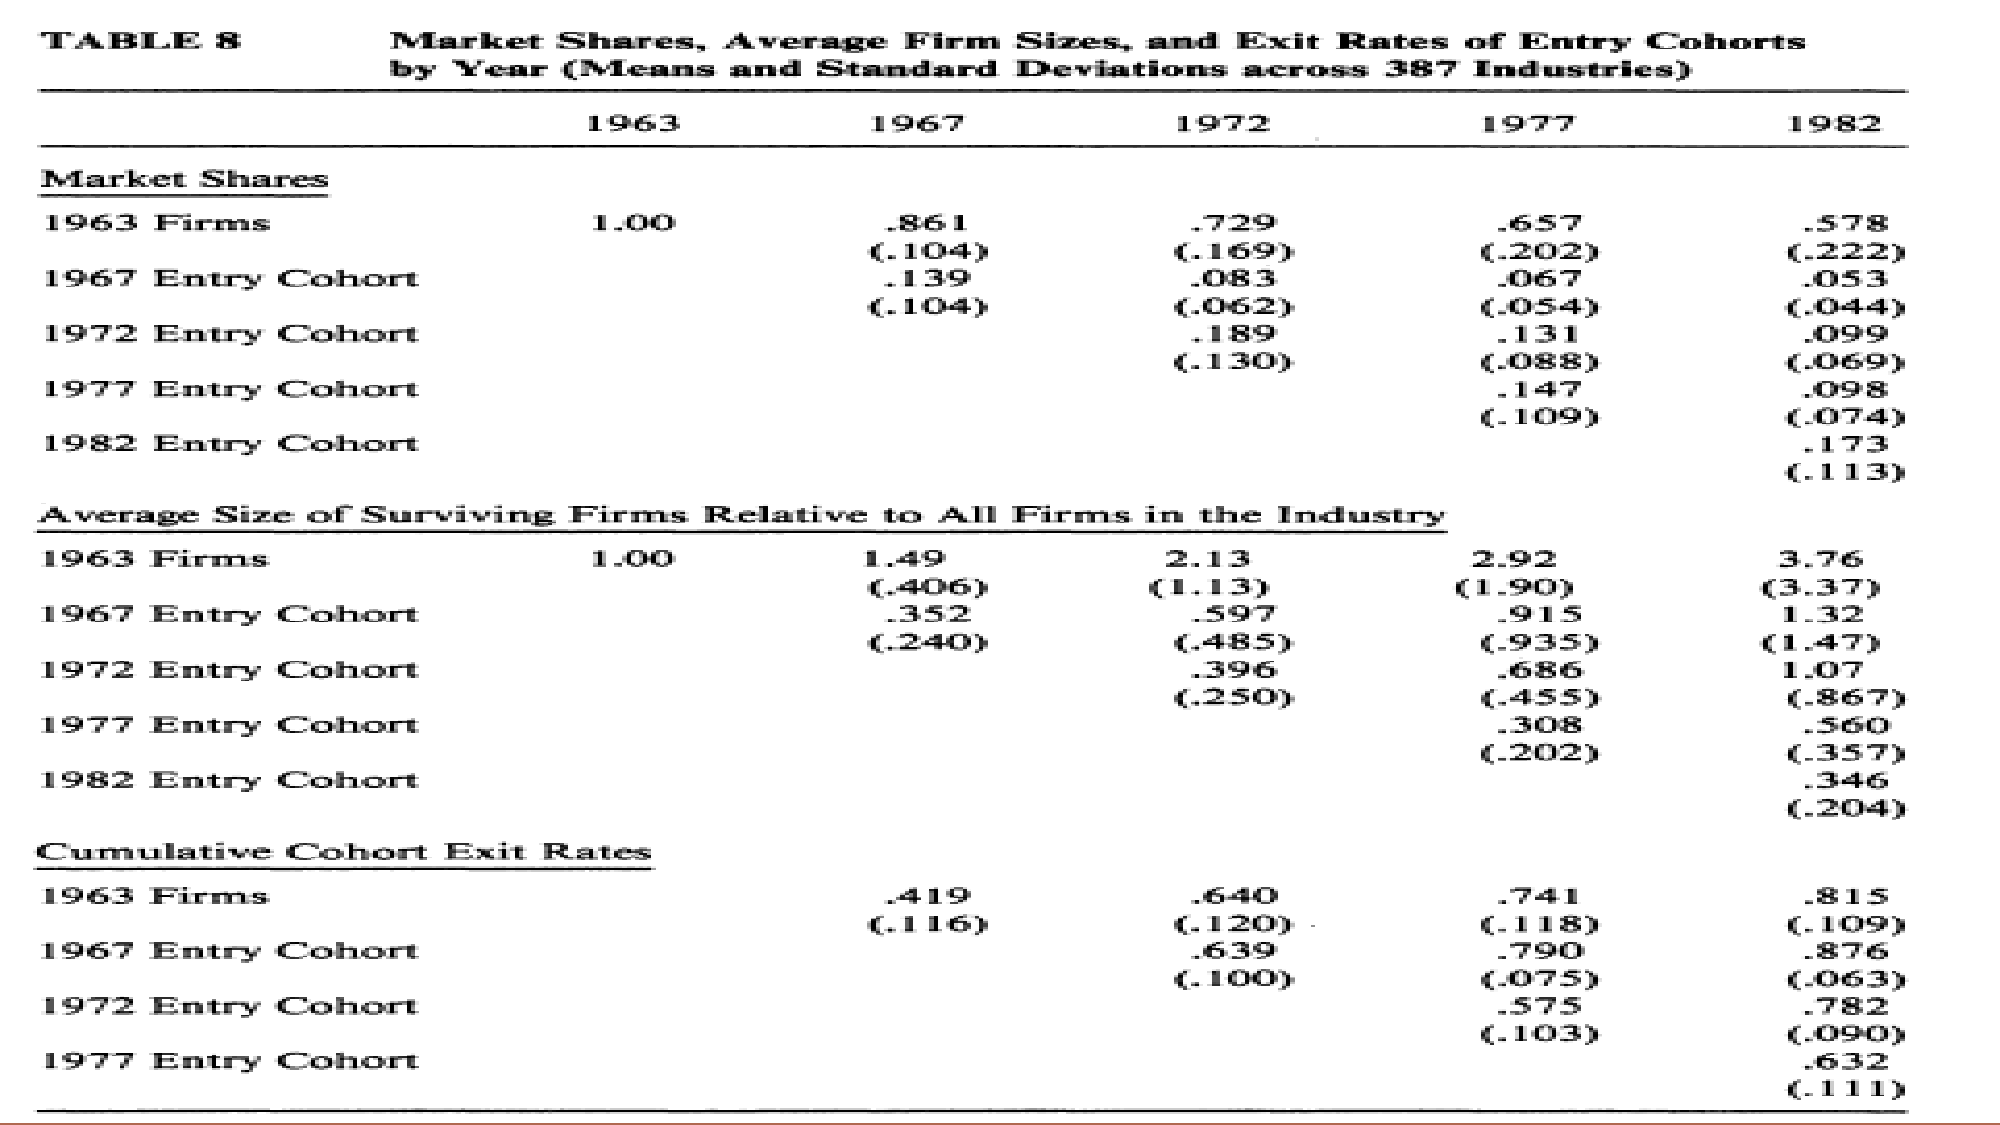
\includegraphics[width=7.5cm,height=8cm]{DRS_T8.pdf}

\end{center}

\end{frame}

\begin{frame}\frametitle{Across-Entry-Type}

 \begin{itemize}
 
 \item About the rate of the number, basic tendency is similar
 
 : DF/NP firms show the smallest decline, while more than a half of DF/PM firm exit within ten years. 
 
 \item In average size, there is large differernce among the types of entry :
 
 DF/NP firms grows to where their average market size is larger than the industry average(largest s.d.).
 
 \item Also in cumulative exit rate, DF/NP firm shows the lowest number.
 
 \end{itemize}

\end{frame}

\begin{frame}

\begin{center}

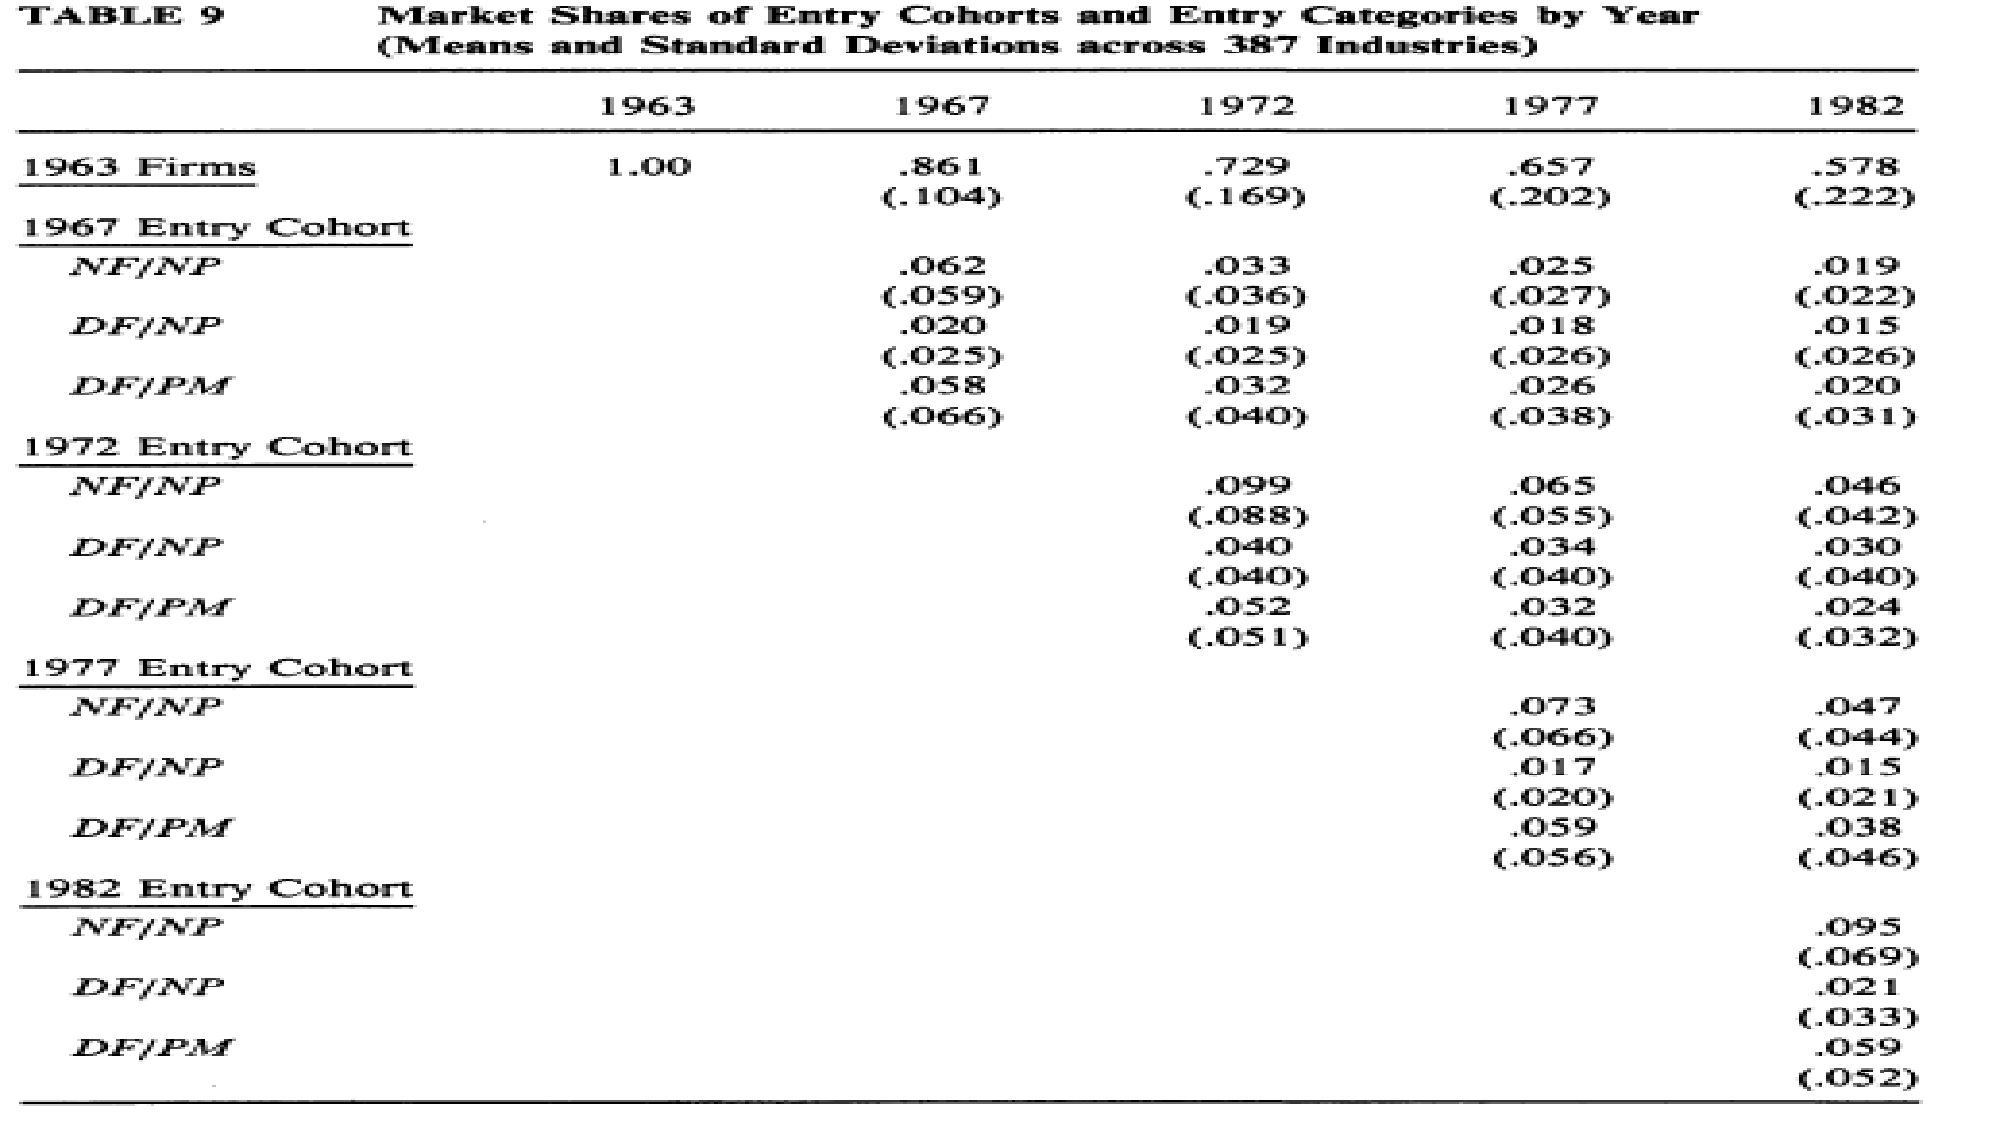
\includegraphics[width=7.25cm,height=8cm]{DRS_T9.pdf}

\end{center}

\end{frame}

\begin{frame}

\begin{center}

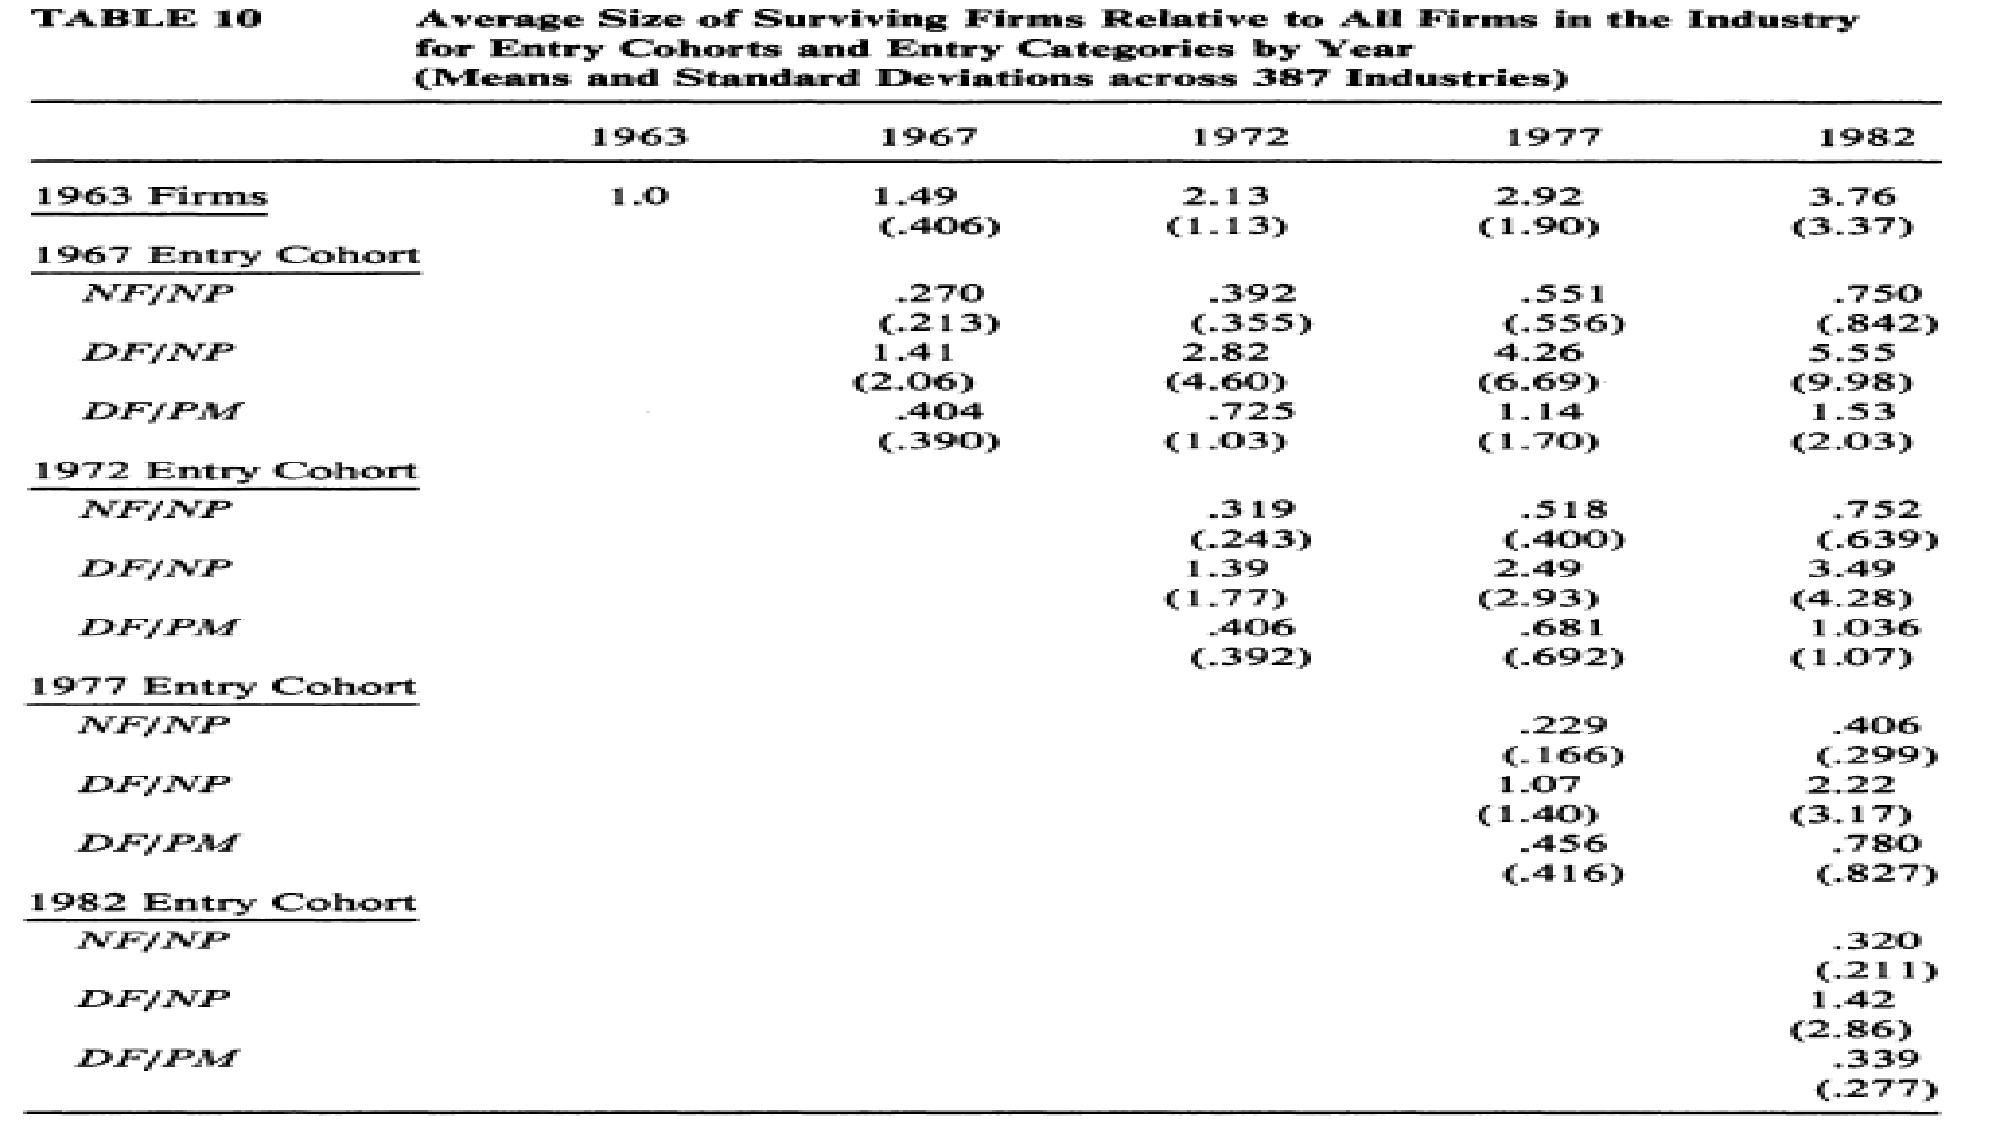
\includegraphics[width=7.5cm,height=8cm]{DRS_T10.pdf}

\end{center}

\end{frame}

\section{Conclusion}
\begin{frame}\frametitle{Conclusion}

 \begin{itemize}
 
 \item Firm-level data from plant-level data provides a summery of the basic patterns of firm entry, growth, and exit.
 
 \item The variation in entry patterns influences on their postentry performance and exit patterns.
 
 \item Further research
 
  \begin{itemize}
  
  \item To identify the charactaristics of industry technology and demand
  
  \item Analyzing within-indusitry competition and long-run evolution of industry structure.
  
  \end{itemize}
 
 \end{itemize}


\end{frame}

\end{document}